\documentclass[10pt, a4paper, twoside, titlepage, usenames,dvipsnames]{report}
\usepackage[a4paper, total={6in, 8in}]{geometry}
\usepackage[section]{placeins}
\usepackage[utf8]{inputenc}
\usepackage{amsfonts, amsmath, amssymb}
\usepackage{physics}
\usepackage{tikz}
\usepackage{float}
\usepackage{graphicx}
\usepackage[style=numeric]{biblatex}

\usepackage[format=plain, font=footnotesize]{caption}
\usepackage[format=plain, font=footnotesize]{subcaption}

\usetikzlibrary{shapes.arrows, fadings, positioning}

\addbibresource{ref.bib}
\renewcommand*{\bibfont}{\footnotesize}
% \pagenumbering{gobble}

\begin{document}

\begingroup
    \centering
    \Large Quasilinear Time Decoding Algorithm for \\Topological Codes with High Error Threshold\\[.5em]
    \large Mark Shui Hu (watermarkhu@gmail.com)\par
\endgroup
\vspace{2em}
One of the most promising approaches for fault-tolerant quantum computation is based on surface quantum error correcting codes \cite{dennis2002topological, kitaev2003fault}. With surface codes, error correction only requires the measurement of local operators on a 2-dimensional lattice of qubits. The measurement outcome, called the syndrome, is passed to the decoding algorithm to deduct the error that has occurred and to supply a correction operator. 
%It is crucial for a decoder to perform fast, where any speed-up of the decoder leads to a reduction of the noise strength as a decreased time between two rounds of correction induces the appearance of fewer errors, and the decoder must be able to keep pace with the clock-speed of the quantum computer.
The resilience against errors can be increased by increasing the system size below a certain threshold physical error rate $p_{th}$. For this, it is essential that the decoder has low time complexity; if the clock-rate of the quantum computer becomes limited by the decoder, the advantages of increasing the system size can be compromised.

Arguably, the most popular decoder for surface codes is the Minimum-Weight Perfect Matching (MWPM) decoder \cite{dennis2002topological}. The basic principle behind this approach is to identify the \emph{lowest weight} error configuration that can produce the syndrome. In general this is a good approximation to the optimal maximum likelihood decoder \cite{}. For a toric code that only suffers random Pauli noise, the optimal code threshold is $p_{th} = 10.9\%$, whereas the MWPM decoder has $p_{th} = 10.3\%$. The MWPM matchings are found by constructing a fully connected graph between nodes of the syndrome, which leads to a superquadratic worst case time complexity of $\mathcal{O}(n^3)$ \cite{kolmogorov2009blossom}.

Many other decoding algorithm that run in polynomial time have been developed \cite{}. A recently proposed decoder called the Union-Find (UF) decoder combines a very low time complexity with a high threshold \cite{delfosse2017linear, delfosse2017almost}. 
The UF decoder maps each (non-trivial) syndrome to a vertex in a non-connected graph on the code lattice, and grows clusters of vertices locally by adding iteratively a layer of edges and vertices to existing clusters until 
all clusters have an even number of syndrome vertices. It then trims the clusters until all vertices are paired and linked by a path, which is the correcting operator. 
By growing the clusters of vertices in order of their sizes, the UF-decoder can be regarded as a heuristic for minimum-weight matching, and has a threshold of $p_{th} = 9.9\%$ for the toric code. 
The complexity of the UF decoder is driven by the merging between clusters. For this the algorithm uses the Union-Find or disjoint-set data structure \cite{tarjan1975efficiency}, which has worst-cast time complexity $\mathcal{O}(n\alpha(n))$, where $\alpha$ is the inverse of Ackermann's function. For any physical feasible amount of qubits, this value is $\alpha(n) \leq 3$, leading to a "Almost-linear" time complexity (see Figure \ref{} for a comparison with MWPM).

%While the time complexity of the UF decoder is impressive, its error threshold has prevented its rise in popularity in the realm of decoding algorithms. Even with the discrepancy of just $0.4\%$ compared to MWPM, it is the latter that most other works use for fidelity and comparison with their own works. 
\textbf{We propose here a modification of the UF decoder that improves the heuristic for minimum-weight matchings. The modified decoder, which we dub the \emph{Balanced Bloom UF decoder} achieves a near MWPM threshold while retaining a quasi linear time complexity.}


The principle of the \emph{Balanced Bloom} decoder is that for a cluster of vertices or a vertex set $\mathcal{V}$, a connected acyclic graph, not all vertices have an equal \emph{matching weight}. Consider the example set $\mathcal{V}_e$, if another vertex $v'$ is connected to the cluster to $v_0$, and a matching is made in $\mathcal{V}_e$, which can simply done by remove some edges as the set is a connected acyclic graph, we are left with edges $(v', v_0), (v_1, v_2)$ which has weight 2. Similarly for vertex $v_2$ the weight is 2. But for $v_1$ we are left with $(v', v_1), (v_0, v_2)$ which has weight 3 (see figure \ref{fig1}). This discrepancy in \emph{potential matching weight} (PMW) is present in any cluster, with increasingly larger differences as the cluster size increases.

The balanced bloom algorithm introduces the node set $\mathcal{N} \subset \mathcal{V}$, also a connected acyclic graph, and consists of the syndrome-node vertices $\sigma$ and a special case junction-node vertices, Each vertex $v \in \mathcal{V}$ is \emph{seeded} in a node $n\in \mathcal{N}$, and for which all vertices seeded in same node (including the node itself) is called the \emph{flower} of a node, where all boundary elements of the flower have the same PMW (see figure \ref{fig2}).

The growth of a cluster, in the context of the UF decoder, is now proceeded by a calculation of the \emph{growth delay} of each node in the cluster. This is done by a 2 depth-first searches of $\mathcal{N}$ (figure \ref{fig3}). In the first traversal the node parity is calculated, the number of children nodes modulo 2, which determines whether a node has larger or smaller delay than its parent, and is only dependant of the parity of its children. In the second traversal the delay is calculated using the node sizes and parities of a node and its parent, and the length of the edge connecting the nodes. This means that node delays can be calculated in constant time in terms of cluster size. The delayed growth of nodes causes the PMW values in the cluster to approach equal value. As the growth of nodes with large PMW is delayed, low PMW nodes are allowed to grow and merge to other clusters with priority, such that the overall matching weight is decreased. We call the growth of a node a bloom, such that our algorithm is named \emph{Balanced Bloom}.

The balanced bloom alteration of the UF decoder has an additional component in the complexity. Due to the merges of clusters, the PMW values in the cluster changes and needs to be recalculated if the cluster is to be grown again. Luckily, by applying some rules during these join operations of node sets, the recalculation of growth delay can be limited a part of the new joint set. We show by a maximization of the join operations that the added balanced bloom has a worst-case time complexity of $\mathcal{O}(n \log n)$, which is still quasilinear.

The error threshold (figure \ref{fig4}) is $p_{th} = 10.25\%$ compared to $10.02\%$ for our implementation of the UF decoder, which is near $10.35\%$ MWPM threshold (thresholds differ from reported value due to changes in cluster sorting, fitting parameters, etc.). The numeric average case time complexity (for a range of error rates in figure \ref{fig5}) is shown to only a linear factor compared to the UF decoder.\\

With the Balanced Bloom algorithm, we would like to show that the UF decoder can be altered in such a way that the heuristic for minimum weight can be improved. Our implementation offers a trade-off in time complexity and error threshold between the UF decoder and the standard MWPM decoder. More alterations may be feasible to further increase the performance of the UF decoder while retaining a low time complexity.

\vspace{2em}
\printbibliography[heading=none]

\tikzstyle{node}=[circle, draw=black, fill=white, minimum size=20pt, line width=1, inner sep= 2pt]
\tikzstyle{nodel}=[circle, draw=black, fill=white, minimum size=5pt, line width=1, inner sep= 0pt]
\tikzstyle{node2}=[circle, draw=black, fill=white, minimum size=8pt, line width=1, inner sep= 0pt, fill=white!70!black]
\tikzstyle{l1}=[line width=1]
\tikzfading[name=fade right, left color=transparent!0, right color=transparent!100]

\begin{figure}[h]
  \centering
     \begin{minipage}[b]{0.3\textwidth}
         \centering
         \begin{tikzpicture}[scale=0.6]

           \node at (-1, -1) {$\mathcal{V}$};
           \draw[l1] (0, 0) -- (4,0);
           \draw[l1, dotted] (-1,0) -- (5,0);
           \draw[l1, dotted] (0,1) -- (0,-1);
           \draw[l1, dotted] (2,1) -- (2,-1);
           \draw[l1, dotted] (4,1) -- (4,-1);
           \node[node] at (0,0) (1) {$v_0$};
           \node[node, draw=green, dashed] at (0,2) (2) {$v_0'$};
           \node[node] at (2,0) (3){$v_1$};
           \node[node, draw=cyan, dashed] at (2,2) (4) {$v_0'$};
           \node[node] at (4,0) (5) {$v_2$};
           \node[node, draw=magenta, dashed] at (4,2) (6) {$v_0'$};

           \draw[l1, dashed, green] (1) -- (2);
           \draw[l1, dashed, green, transform canvas={yshift=2pt}] (3) -- (5);
           \draw[l1, dashed, cyan] (3) -- (4);
           \draw[l1, dashed, cyan, transform canvas={yshift=-2pt}] (1) -- (3) -- (5);
           \draw[l1, dashed, magenta] (5) -- (6);
           \draw[l1, dashed, magenta, transform canvas={yshift=2pt}] (3) -- (1);

         \end{tikzpicture}
         \captionof{figure}{Unbalanced matching weight in cluster vertex set $\mathcal{V}$. The matching edges (dashed) correspond to the position of $v'$. }\label{fig1}
     \end{minipage}
     \hfill
     \begin{minipage}[b]{0.3\textwidth}
         \centering
         \begin{tikzpicture}[scale=0.6]
           \node[node, fill=white!70!green] at (0,0) (0) {$\sigma_0$};
           \node[node, fill=white!70!cyan] at (2,0) (1) {$\sigma_1$};
           \node[node, fill=white!70!black, path fading=fade right] at (4,0) (5) {$\sigma_2$};
           \node[node] at (-2,0) (2) {$v_3$};
           \node[node] at (0,2) (3) {$v_4$};
           \node[node] at (0,-2) (4) {$v_5$};
           \draw[l1] (1) -- (0) -- (3);
           \draw[l1] (2) -- (0) -- (4);
           \draw[l1, dotted] (2, 1.5) -- (1) -- (2,-1.5);
           \draw[l1] (1) -- (5);
           \fill[color=green!50!white, opacity=0.3] (0,3) arc (90:225:1) arc (45:-135:.4142) arc (45:315:1) arc (135:-45:.4142) arc (135:405:1) arc (225:135:.4142) arc (-45:45:1) arc (225:135:.4142) arc (-45:90:1) -- cycle;
           \fill[color=cyan!50!white, opacity=0.3] (2,1) arc (90:450:1);

           \node at (-2, 2.5) {$\mathcal{V}$};
           \node at (2, -2.5) {$\mathcal{N}:$};

           \node[nodel, fill=white!70!green] at (2.8, -2.55) (d) {};
           \node[nodel, fill=white!70!cyan] at (3.3, -2.55) (e) {};
           \node[nodel, fill=white!70!black] at (3.8, -2.55) (f) {};
           \draw[l1] (d) -- (e) -- (f);
           \draw[l1, path fading=fade right] (f) -- (4.3, -2.55);
         \end{tikzpicture}
         \captionof{figure}{A node set $\mathcal{N}$ vs. a vertex set $\mathcal{V}$, both representing the cluster. The shaded area is the flower of a node.}\label{fig2}
     \end{minipage}
     \hfill
     \begin{minipage}[b]{0.3\textwidth}
         \centering
         \begin{tikzpicture}
           \node[node2] (a) at (1, 3) {};
           \node[node2] (b) at (1, 2) {};
           \node[node2] (c) at (1, 1) {};
           \node[node2] (d) at (1, 0) {};
           \node[node2] (e) at (0, 1) {};
           \node[node2] (f) at (0, 0) {};
           \node[node2] (g) at (2, 2) {};
           \node[node2] (h) at (2, 1) {};
           \node[node2] (i) at (2, 0) {};
           \draw[l1] (a) -- (b) -- (c) -- (d);
           \draw[l1] (b) -- (e);
           \draw[l1] (c) -- (f);
           \draw[l1] (c) -- (i);
           \draw[l1] (a) -- (g) -- (h);

           \draw[l1, ->, color=cyan] (0, 1.3) -- +(45:0.85) arc (-45:0:.5) -- +(90:.6);
           \draw[l1, ->, color=cyan] (0, 0.3) -- +(45:0.85) arc (-45:0:.5) -- +(90:.2);
           \draw[l1, ->, color=cyan] (0.75,0.2) -- +(90:.3);
           \draw[l1, ->, color=cyan] (1.5,0.2) -- +(135:.4);
           \draw[l1, ->, color=cyan] (1.75,1.2) -- +(90:0.5) arc (0:45:.5) -- +(135:0.4);
           \draw[l1, ->, color=magenta] (1.4, 3) -- +(-45:1.1) arc (45:0:0.5) -- +(-90:0.7);
           \draw[l1, ->, color=magenta] (1.3, 2.1) -- +(-90:0.9) arc (180:225:.5) -- +(-45:0.7);
           \draw[l1, ->, color=magenta] (0.6, 1.3) -- +(225:.3);
           \draw[l1, ->, color=magenta] (0.6, 0.3) -- +(225:.3);
           \draw[l1, ->, color=magenta] (1.3, 0.3) -- +(-90:.2);
           \node[text=cyan] at (0,2.2) {Parity};
           \node[text=magenta] at (2.6,2.8) {Delay};
           \node at (0,3) {$\mathcal{N}$};
         \end{tikzpicture}
         \captionof{figure}{Two depth-first searches on $\mathcal{N}$ to compute node parities (head recursively) and delays (tail recursively).}\label{fig3}
     \end{minipage}
\end{figure}

\begin{figure}
    \centering
    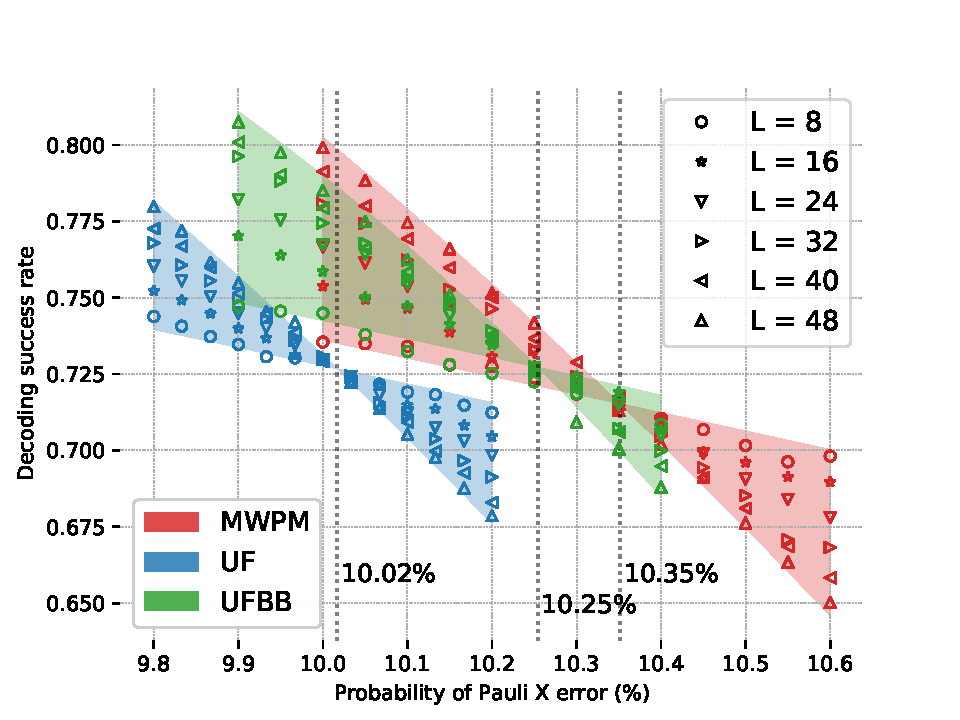
\includegraphics[width=0.55\textwidth]{threshold.pdf}
    \caption{Decoder success rate and threshold.}\label{fig4}
\end{figure}
\begin{figure}
    \centering
    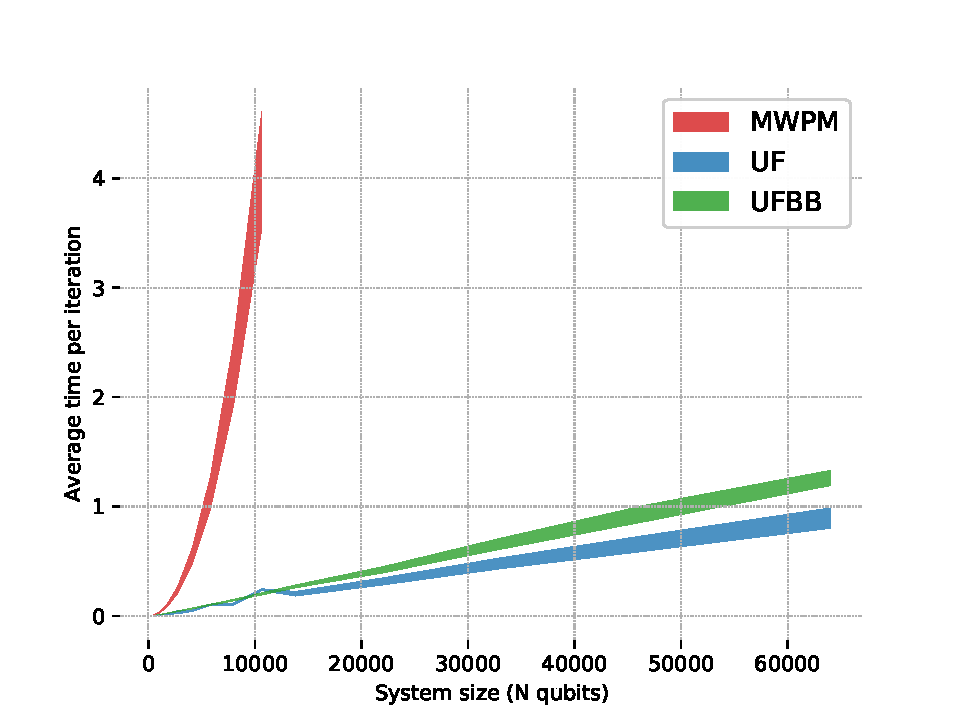
\includegraphics[width=0.55\textwidth]{time.pdf}
    \caption{Decoder performance in computation time.}\label{fig5}
\end{figure}

\end{document} 